% ============================================================
% FINAL PROJECT REPORT - ENGLISH VERSION
% Project 05: Audiobook Generation (TTS Front-End)
% Course: CSC15012 - Applications of NLP in Industry
% Student: Le Dinh Minh Quan - 23127460 - 23CNTThuc
% ============================================================
\documentclass[12pt,a4paper]{article}

\usepackage[utf8]{inputenc}
\usepackage{geometry}
\geometry{left=2.3cm, right=2.3cm, top=2.5cm, bottom=2.5cm}
\usepackage{setspace}
\setstretch{1.25}
\usepackage{graphicx}
\usepackage{float}
\usepackage{booktabs}
\usepackage{longtable}
\usepackage{tabularx}
\usepackage{array}
\usepackage{hyperref}
\hypersetup{colorlinks=true, linkcolor=blue, urlcolor=blue, citecolor=blue, breaklinks=true}
\usepackage{xurl}
\usepackage{seqsplit}
\usepackage{listings}
\usepackage{xcolor}
\usepackage{amsmath}
\usepackage{caption}
\usepackage{subcaption}
\usepackage{enumitem}
\usepackage{fancyhdr}
\usepackage{tikz}
\usetikzlibrary{shapes.geometric, arrows.meta, positioning, fit, backgrounds, shadows}

% --- Make long inline code / paths break gracefully ---
\sloppy
\tolerance=2000
\emergencystretch=3em
\hbadness=10000
\setlength{\parskip}{0.15em}

% Helper for breakable monospaced paths
\newcommand{\bpath}[1]{\seqsplit{#1}}
\newcommand{\btt}[1]{\texttt{\seqsplit{#1}}}

% New column type for tabularx: left-aligned and ragged-right with breaking
\newcolumntype{L}{>{\raggedright\arraybackslash}X}

\lstset{
  basicstyle=\ttfamily\small,
  breaklines=true,
  frame=single,
  backgroundcolor=\color{gray!10},
  keywordstyle=\color{blue},
  commentstyle=\color{green!60!black},
  stringstyle=\color{red!70!black},
  showstringspaces=false,
  tabsize=2
}

\pagestyle{fancy}
\fancyhf{}
\fancyhead[L]{\small CSC15012 -- Final Project Report}
\fancyhead[R]{\small Le Dinh Minh Quan -- 23127460}
\fancyfoot[C]{\thepage}

% ============================================================
\begin{document}

% --- TITLE PAGE ---
\begin{titlepage}
\centering
\vspace*{0.5cm}

% HCMUS LOGO: upload logo_hcmus.png to Overleaf and uncomment the next line
\IfFileExists{logo_hcmus.png}{\includegraphics[width=3.5cm]{logo_hcmus.png}\\[0.5cm]}{}

{\large \textbf{VIETNAM NATIONAL UNIVERSITY HO CHI MINH CITY}}\\[0.3cm]
{\Large \textbf{UNIVERSITY OF SCIENCE}}\\[0.3cm]
{\large Faculty of Information Technology}\\[1.5cm]

{\LARGE \textbf{FINAL PROJECT REPORT}}\\[0.5cm]
{\large Course: \textbf{CSC15012 -- Applications of Natural Language\\ Processing in Industry}}\\[1.5cm]

{\Large \textbf{Project 05:}}\\[0.3cm]
{\Large \textbf{Audiobook Generation (TTS Front-End)}}\\[0.3cm]
{\large A Trainable Text-Normalization Model with a Deterministic Agentic Pipeline}\\[2cm]

\begin{tabular}{ll}
\textbf{Student:} & Le Dinh Minh Quan \\
\textbf{Student ID:} & 23127460 \\
\textbf{Class:} & 23CNTThuc \\
\end{tabular}

\vfill
{\large Ho Chi Minh City, 2026}
\end{titlepage}

\tableofcontents
\newpage

% ============================================================
\section{Introduction}
% ============================================================

Turning long-form documents (EPUB / PDF / TXT / Markdown) into listenable audiobooks fails on two fronts. First, \textbf{text normalization}: a naive text-to-speech (TTS) engine reads \texttt{\$5.2M}, \texttt{1984}, \texttt{Dr.}, \texttt{Chapter IV}, \texttt{3/4}, and \texttt{9:45 AM} literally or wrongly, which is jarring and sometimes \emph{unrecoverable} for a listener. Second, \textbf{production orchestration}: chapter detection, sentence-safe chunking, multi-voice routing, loudness mastering, and chapter-marked exports are tedious and error-prone.

This project implements a complete \textbf{Audiobook Generation} system end-to-end, including:
\begin{itemize}
  \item A \textbf{trainable Text-Normalization (TN) seq2seq model} (the NLP-heavy core) that converts \emph{written} text into \emph{spoken} form across 16 semiotic classes
  \item A pretrained neural \textbf{TTS backend} (SpeechT5) that produces the audio
  \item A deterministic \textbf{agentic finite-state machine (FSM)} with four decision points that orchestrates the whole \texttt{document $\rightarrow$ audiobook} pipeline
  \item Production-ready deployment: a FastAPI REST API, a Gradio demo UI, a CLI, batch processing, and Docker, plus a one-button Colab H100 autopilot
\end{itemize}

The hard, NLP-heavy part of audiobook production is text normalization, so it is the part that is trained and evaluated rigorously; the audio is produced by an off-the-shelf neural TTS, and the agent binds the stages together with an auditable trace and a reproducible \texttt{manifest.json}.

\textbf{Project Resources (public):}
\begin{itemize}\setlength\itemsep{0.15em}
  \item \textbf{GitHub repository (source code):} \url{https://github.com/ledinhminhquan/05_Audiobook_Generation}
  \item \textbf{Reference inspiration:} \texttt{denizsafak/abogen} -- \url{https://github.com/denizsafak/abogen}
  \item \textbf{Deployment artifacts:} FastAPI REST API + Gradio UI + CLI + Docker + one-button Colab H100 autopilot notebook (all in the repository under \texttt{src/audiobook\_ai/api/}, \texttt{deploy/}, and \texttt{notebooks/})
\end{itemize}

\noindent\textit{Deployment note:} the system is fully \textbf{deployable} (REST API, Gradio UI, CLI, Docker image, and a Hugging Face Space wrapper) and runs CPU-only with zero paid API. The verified, headline numbers in this report are the \textbf{offline, synthetic-spine} results checked on the developer machine; the full corpus training run is performed by the one-button Colab H100 autopilot notebook.

% ============================================================
\section{Business Problem Definition}
% ============================================================

\subsection{Context and Motivation}

Audiobook demand keeps rising, but professional human narration is slow and expensive, and most text catalogs are never converted to audio at all. The blockers are:
\begin{itemize}
  \item \textbf{Cost}: studio narration is expensive per finished audio-hour, putting audiobook production out of reach for independent authors and back-catalog titles.
  \item \textbf{Accessibility}: sight-impaired, dyslexic, and time-constrained readers cannot access text-only documents.
  \item \textbf{Scale}: chapter detection, sentence-safe chunking, multi-voice routing, loudness mastering, and chaptered exports are tedious and error-prone to do by hand at catalog scale.
\end{itemize}

\subsection{Target Users and Stakeholders}

\begin{itemize}
  \item \textbf{Readers with disabilities}: sight-impaired and dyslexic readers gain spoken access to text-only documents.
  \item \textbf{Commuters / time-constrained learners}: listening replaces reading; chapter 1 streams while later chapters render.
  \item \textbf{Independent authors}: audiobook production at compute-only cost, far below studio narration.
  \item \textbf{Publishers}: faster catalog conversion of back-catalog titles, with chaptered \texttt{.m4b} and synchronized \texttt{.srt} produced automatically.
  \item \textbf{Developers}: an easy-to-integrate REST API and CLI for programmatic conversion.
\end{itemize}

\subsection{Problem Statement}

Given a document (EPUB / PDF / TXT / Markdown), the system must:
\begin{enumerate}
  \item \textbf{Normalize written text to spoken form in context}: numbers, dates, money, abbreviations, Roman numerals, units, fractions, times, telephone numbers, and URLs across 16 semiotic classes.
  \item \textbf{Orchestrate production}: parse $\rightarrow$ detect chapters $\rightarrow$ segment and classify $\rightarrow$ normalize $\rightarrow$ route voices $\rightarrow$ synthesize $\rightarrow$ audio-QA $\rightarrow$ stitch and master $\rightarrow$ export.
  \item \textbf{Produce an auditable, reproducible build} of mastered, chaptered audio (\texttt{.wav} / \texttt{.mp3} / \texttt{.m4b}) plus read-along \texttt{.srt} and a \texttt{manifest.json}.
\end{enumerate}

\subsection{Why NLP is Required}

Text normalization is fundamentally a \textbf{contextual language} problem. The same surface form maps to different spoken forms depending on surrounding words: \texttt{St.}\ is ``Street'' in ``Main St.''\ but ``Saint'' in ``St.\ Patrick''; \texttt{1984} is a year in ``in 1984'' but a count in ``1984 people''; \texttt{IV} is ``four'' in ``Chapter IV'' but ``I-V'' in ``IV drip''. A context-blind rule engine cannot resolve these, so a learned, context-aware sequence-to-sequence model is required.

\subsection{Success Metrics}

\begin{table}[H]
\centering
\caption{System success metrics (business + technical)}
\begin{tabularx}{\linewidth}{@{} l L l @{}}
\toprule
\textbf{Type} & \textbf{Metric} & \textbf{Target} \\
\midrule
Business & Cost per finished audio-hour & $\ll$ human narration (compute-only) \\
Business & Time-to-first-audio (stream chapter 1) & A few seconds \\
Business & Unrecoverable mis-read rate per chapter & $\rightarrow 0$ \\
Technical & TN sentence exact-match (EM) accuracy & Beat the rule baseline \\
Technical & TN macro per-class accuracy (16 classes) & Beat the rule baseline \\
Technical & Audio-QA first-try pass rate & High; bounded re-synth $N=2$ \\
Technical & Loudness conformance & $-18$ LUFS / $-3$ dBTP (ACX-safe) \\
Technical & Real-Time Factor (RTF) & $\sim$0.1 on GPU; reported per job \\
\bottomrule
\end{tabularx}
\end{table}

% ============================================================
\section{Development Infrastructure \& Tooling}
% ============================================================

\subsection{Repository Structure}

The project follows a production-ready Python package layout under \texttt{src/audiobook\_ai/}, mirroring the public GitHub repository \url{https://github.com/ledinhminhquan/05_Audiobook_Generation}. Stages of the \texttt{document $\rightarrow$ audiobook} pipeline map one-to-one onto subpackages (\texttt{data}, \texttt{models}, \texttt{synthesis}, \texttt{training}, \texttt{agent}, \texttt{api}, \texttt{analysis}, \texttt{autoreport}, \texttt{monitoring}, \texttt{automation}, \texttt{grading}), and twelve rubric-aligned docs live under \texttt{docs/}.

\begin{lstlisting}[basicstyle=\ttfamily\footnotesize]
05_Audiobook_Generation/
|-- src/audiobook_ai/                 # Python package
|   |-- config.py  cli.py  logging_utils.py
|   |-- data/                         # data + corpus
|   |   |-- document.py               # EPUB/PDF/TXT/MD parsing (ebooklib/PyMuPDF)
|   |   |-- tn_corpus.py              # synthetic (written,spoken) generator (16 classes)
|   |   |-- dataset.py  samples.py  download_dataset.py
|   |-- models/                       # normalizers + registry
|   |   |-- expanders.py              # num2words / inflect verbalizers
|   |   |-- baseline_rules.py         # context-BLIND rule baseline (the bar to beat)
|   |   |-- normalizer.py             # trained ByT5-small inference
|   |   +-- model_registry.py         # tn_meta.json + latest pointer + repo@revision pins
|   |-- synthesis/                    # TTS + audio
|   |   |-- tts_backend.py            # SpeechT5 (+ Kokoro/Parler/pyttsx3/Placeholder)
|   |   |-- voices.py  stitch.py  subtitles.py
|   |-- training/                     # train, evaluate, tune
|   |   |-- train_normalizer.py       # HuggingFace Seq2SeqTrainer recipe
|   |   |-- evaluate.py  tune.py
|   |-- agent/                        # deterministic FSM (mandatory agentic component)
|   |   |-- state.py                  # append-only versioned JobState
|   |   |-- policy.py                 # transitions + D1-D4 decision logic
|   |   |-- tools.py                  # pydantic tool contracts
|   |   |-- llm_orchestrator.py       # optional Anthropic brain (off by default)
|   |   +-- narrator_agent.py         # driver
|   |-- api/                          # serving surfaces
|   |   |-- main.py                   # FastAPI: /healthz /readyz /normalize /synthesize
|   |   |-- ui.py                     # Gradio web demo
|   |   |-- app_combined.py           # combined ASGI app (UI mounted at /ui)
|   |   +-- schemas.py  dependencies.py
|   |-- analysis/ autoreport/ monitoring/ automation/ grading/
|-- configs/                          # train.yaml, infer YAMLs, GPU profiles
|-- docs/                             # 12 rubric-aligned docs (.md) + DESIGN_BRIEF
|-- tests/                            # CPU-only pytest (no model/network downloads)
|-- notebooks/                        # Colab H100 AUTOPILOT notebook + COLAB_GUIDE
|-- deploy/                           # Dockerfile (api/worker), compose, hf_space/app.py
|-- data/ models/ app/ sample_data/   # corpus, checkpoints, sample book
|-- Dockerfile  docker-compose.yml  Makefile
|-- pyproject.toml  requirements*.txt
|-- LICENSE (MIT)  README.md
\end{lstlisting}

\subsection{Technology Stack}

\begin{table}[H]
\centering
\caption{Technology stack}
\small
\begin{tabularx}{\linewidth}{@{} l L @{}}
\toprule
\textbf{Component} & \textbf{Technology} \\
\midrule
Language & Python 3.12 \\
Version Control & Git + GitHub (public repo) \\
ML Framework & PyTorch (CUDA), HuggingFace Transformers + Datasets, \texttt{Seq2SeqTrainer} \\
Trainable TN model & \texttt{google/byt5-small} (byte/char-level, $\sim$300M params; Apache-2.0) \\
TN fallback model & \texttt{google-t5/t5-small} (60.5M params, T4-friendly; Apache-2.0) \\
TN baseline & regex spans + abbreviation dict + \texttt{num2words}/\texttt{inflect} (context-blind) \\
TTS (primary) & \texttt{microsoft/speecht5\_tts} + \texttt{microsoft/speecht5\_hifigan} (MIT) \\
Speaker voices & \texttt{Matthijs/cmu-arctic-xvectors} (7 speakers; MIT) \\
TTS (optional) & \texttt{hexgrad/Kokoro-82M}, \texttt{parler-tts/parler-tts-mini-v1} (Apache-2.0) \\
Parsing & \texttt{ebooklib} (EPUB), \texttt{PyMuPDF} + \texttt{pdfplumber} (PDF), \texttt{pysbd} (sentences) \\
Audio & \texttt{soundfile}, \texttt{pydub} + \texttt{ffmpeg}, \texttt{pyloudnorm}, \texttt{mutagen} \\
API / UI & FastAPI + Uvicorn; Gradio web demo (mounted at \texttt{/ui}) \\
Containerization & Docker + Docker Compose (api CPU + worker GPU); Hugging Face Space \\
Training GPU & Google Colab H100/A100/L4/T4 (auto-profiled; bf16/tf32 on H100) \\
\bottomrule
\end{tabularx}
\end{table}

\subsection{Training \& Autopilot Workflow}
\label{subsec:workflow}

The end-to-end training-to-report workflow is automated by the Colab notebook \texttt{Audiobook\_AI\_Colab\_Training\_H100\_AUTOPILOT.ipynb}. It mounts Drive, installs Colab-safe dependencies (never touches \texttt{torch}), \textbf{auto-profiles the GPU} (H100/A100/L4/T4 $\rightarrow$ batch + precision, effective batch held constant at 256), trains resume-safely, evaluates against the rule baseline, runs the agent, and generates the report and slides.

\begin{figure}[H]
\centering
\resizebox{\linewidth}{!}{%
\begin{tikzpicture}[
  node distance=0.32cm,
  step/.style={rectangle, draw=black!60, rounded corners=2pt, thick,
              text width=13.5cm, inner sep=5pt, minimum height=0.75cm,
              align=center, font=\footnotesize},
  setup/.style={step, fill=gray!15},
  train/.style={step, fill=orange!15},
  eval/.style={step, fill=blue!15},
  deploy/.style={step, fill=green!15},
  arrow/.style={-{Stealth[length=2mm]}, thick}
]

\node[setup] (s1) {\textbf{1. Setup (Colab)}: mount Drive, clone repo, install Colab-safe deps (never touch \texttt{torch}), set \texttt{ARTIFACTS\_DIR}};
\node[setup, below=of s1] (s2) {\textbf{2. GPU auto-profile}: \texttt{torch.cuda.get\_device\_name} $\rightarrow$ H100/A100/L4/T4 batch + precision; effective batch held at \textbf{256}};
\node[setup, below=of s2] (s3) {\textbf{3. Build synthetic TN corpus}: \texttt{tn\_corpus.py} $\rightarrow$ train 60k / val 4k / test 4k / hard 1.5k (dedup, leakage-free, PLAIN $\le$30\%)};
\node[train, below=of s3] (s4) {\textbf{4. Train ByT5-small} (resume-safe): \texttt{Seq2SeqTrainer}, bf16+tf32, lr 5e-4, cosine, label smoothing 0.1, early stop (patience 4)};
\node[eval, below=of s4] (s5) {\textbf{5. Evaluation}: rule baseline vs.\ neural on \texttt{test} + \texttt{hard}; sentence EM, macro/per-class accuracy, unrecoverable-error count};
\node[eval, below=of s5] (s6) {\textbf{6. Run the agent FSM} on the sample book: all 4 decisions (D1--D4) fire; latency/RTF benchmark + audio-QA report};
\node[deploy, below=of s6] (s7) {\textbf{7. Auto-gen report \& slides}: \texttt{report.pdf} + \texttt{slides.pptx} from artifacts};
\node[deploy, below=of s7] (s8) {\textbf{8. Self-grade}: \texttt{audiobook-ai grade} rubric-completeness check + submission bundle};

\foreach \a/\b in {s1/s2, s2/s3, s3/s4, s4/s5, s5/s6, s6/s7, s7/s8}
  \draw[arrow] (\a) -- (\b);

\end{tikzpicture}%
}
\caption{Eight-step autopilot workflow inside the Colab notebook. Training auto-resumes from the last checkpoint; the effective batch size is held at 256 across all GPU profiles; every run writes an auditable \texttt{manifest.json}.}
\label{fig:workflow}
\end{figure}

\paragraph{Key notebook characteristics:}
\begin{itemize}\setlength\itemsep{0.15em}
  \item \textbf{One-button Run-All}: corpus build + training + evaluation + agent run + report/slides in a single execution.
  \item \textbf{GPU auto-profile}: per-device batch and precision are selected from the GPU name (H100/A100/L4/T4) while the \emph{effective} batch size stays 256, so optimization is stable regardless of hardware.
  \item \textbf{Resume-safe}: training resumes from the last checkpoint via \texttt{get\_last\_checkpoint} if Colab disconnects.
  \item \textbf{Never touches torch}: Colab's pre-installed CUDA \texttt{torch} is left intact to avoid environment breakage.
  \item \textbf{CPU floor}: a deterministic \texttt{PlaceholderTTS} and the rule normalizer mean the pipeline (and the smoke run) work with no model weights and no GPU.
\end{itemize}

% ============================================================
\section{Data Management}
% ============================================================

\subsection{Data Source}

The only \emph{trained} component is the Text-Normalization model, and its training data is a reproducible \textbf{synthetic corpus generator} (\texttt{src/audiobook\_ai/data/tn\_corpus.py}). Synthetic data is the \textbf{primary} source by necessity, not convenience:

\begin{itemize}\setlength\itemsep{0.15em}
  \item There is \textbf{no permissively-licensed English TN-Challenge mirror on the Hugging Face Hub} -- the canonical ids \texttt{google/text\_normalization} and \texttt{cestwc/text-normalization} return \textbf{404}. The only English-adjacent set is GPL-licensed ITN data with a broken viewer.
  \item The generator is deterministic and version-controlled, so any grader can rebuild the exact corpus from source with no missing or license-encumbered download.
  \item \textbf{Optional real-data loader} (opt-in, local) and an \textbf{optional eval sanity set} \texttt{DigitalUmuganda/Text\_Normalization\_Challenge\_Unittests\_Eng\_Fra} (VERIFIED on the Hub) are available for an external cross-check, not for the headline numbers.
\end{itemize}

\subsection{The 16 Semiotic Classes and Injected Ambiguity}

The generator emits context-rich \texttt{(written, spoken)} sentence pairs covering all 16 semiotic classes: \texttt{PLAIN, PUNCT, CARDINAL, ORDINAL, DECIMAL, DIGIT, MONEY, MEASURE, DATE, TIME, FRACTION, TELEPHONE, ELECTRONIC, ABBREV, ROMAN, VERBATIM}. Crucially it embeds each token in a carrier sentence and \textbf{injects ambiguity} that a context-blind ruleset cannot resolve:

\begin{table}[H]
\centering
\caption{Examples of injected ambiguity (context decides the spoken form)}
\small
\begin{tabularx}{\linewidth}{@{} l L L @{}}
\toprule
\textbf{Written} & \textbf{Context A $\rightarrow$ spoken} & \textbf{Context B $\rightarrow$ spoken} \\
\midrule
\texttt{St.} & ``Main \textbf{St.}'' $\rightarrow$ ``Main Street'' & ``\textbf{St.}\ Patrick'' $\rightarrow$ ``Saint Patrick'' \\
\texttt{1984} & ``\textbf{1984} people'' $\rightarrow$ ``one thousand nine hundred eighty four'' (count) & ``in \textbf{1984}'' $\rightarrow$ ``nineteen eighty four'' (year) \\
\texttt{IV} & ``Chapter \textbf{IV}'' $\rightarrow$ ``four'' (Roman) & ``\textbf{IV} drip'' $\rightarrow$ ``I V'' (verbatim) \\
\bottomrule
\end{tabularx}
\end{table}

\subsection{Data Splits}

\begin{table}[H]
\centering
\caption{Default synthetic-corpus splits (English only; total $\approx$69,500 pairs)}
\begin{tabular}{llr}
\toprule
\textbf{Split} & \textbf{Role} & \textbf{Size} \\
\midrule
train & model training & 60,000 \\
val & early stopping / model selection & 4,000 \\
test & held-out general evaluation & 4,000 \\
hard & held-out ambiguity-stress slice & 1,500 \\
\bottomrule
\end{tabular}
\end{table}

\subsection{Preprocessing and Anti-Leakage Discipline}

\begin{itemize}\setlength\itemsep{0.15em}
  \item \textbf{Unicode NFC} normalization (visually-identical strings share one byte representation -- important for the byte-level model).
  \item \textbf{Task prefix} \texttt{"normalize: "} on every input (the T5/ByT5 convention).
  \item \textbf{Deduplication before splitting} -- identical \texttt{(written, spoken)} pairs cannot appear in two splits.
  \item \textbf{Leakage-free splits} -- no validation or test input appears in train.
  \item \textbf{PLAIN capped at $\approx$30\%} so the headline number is not inflated by trivial pass-through tokens and rare classes get real representation.
\end{itemize}

\subsection{License Hygiene (Non-Commercial Flags)}

The commercial path uses \textbf{only MIT/Apache-2.0} model ids. The following are explicitly \textbf{flagged as non-commercial and excluded from the default path}: \texttt{coqui/XTTS-v2} (CPML, voice-clone), \texttt{facebook/mms-tts-eng} (CC-BY-NC-4.0), \texttt{SWivid/F5-TTS} (CC-BY-NC-4.0), and the \texttt{MahmoudAshraf/mms-300m-1130-forced-aligner} (CC-BY-NC; swap to the torchaudio MMS aligner for commercial use). GPL TN data is likewise excluded.

% ============================================================
\section{Model Selection \& Optimization}
% ============================================================

\subsection{What is Actually Being Selected}

Only one part of the pipeline is a genuinely \emph{learned} NLP problem: \textbf{text normalization}. The audio is produced by a pretrained TTS; the orchestration is a deterministic FSM. So the model selected and trained is the TN model, and it must be robust to numbers, symbols, dates, currencies, and out-of-vocabulary (OOV) tokens.

\subsection{Candidates and the Chosen Model}

\begin{table}[H]
\centering
\caption{Model candidates for the TN core}
\small
\begin{tabularx}{\linewidth}{@{} l l L @{}}
\toprule
\textbf{Option} & \textbf{Role} & \textbf{Decision} \\
\midrule
Rule-only (\texttt{baseline\_rules.py}) & regex + dict + \texttt{num2words} & Baseline + runtime guardrail; context-blind, not the model \\
\texttt{google-t5/t5-small} (60.5M) & subword T5 & Fallback on small GPUs (T4); subword fragments numbers/OOV \\
\texttt{google/flan-t5-small} & instruction-tuned subword & Rejected; same subword limit, larger, marginal gain \\
\textbf{\texttt{google/byt5-small}} ($\sim$300M) & \textbf{byte/char-level T5} & \textbf{Selected.} No OOV, char-robust, faithful transduction \\
\bottomrule
\end{tabularx}
\end{table}

\textbf{Why byte-level wins.} TN is fundamentally about characters: a model must distinguish \texttt{1984} (year) from \texttt{1984 people} (count), expand \texttt{\$5.2M}, and read Roman numerals in \texttt{Chapter IV}. ByT5 operates over raw UTF-8 bytes, so (a) there is \textbf{no OOV} -- every novel number/symbol is representable; (b) it is \textbf{robust to noisy/adversarial tokens}, odd spacing, and garbled OCR; (c) it does \textbf{faithful transduction} at the character granularity the task demands. Both ByT5-small and the t5-small fallback are Apache-2.0, keeping the commercial path on MIT/Apache ids only.

\subsection{Training Configuration}

\begin{table}[H]
\centering
\caption{Final training configuration (HuggingFace \texttt{Seq2SeqTrainer})}
\begin{tabular}{ll}
\toprule
\textbf{Parameter} & \textbf{Value} \\
\midrule
Model & \texttt{google/byt5-small} ($\sim$300M; fallback \texttt{t5-small}) \\
Task prefix & \texttt{"normalize: "} \\
Max source / target length & 256 / 256 (token-level 128/128; t5-small 192/192) \\
Effective batch size & 256 (held constant across all GPUs) \\
Per-device batch / grad-accum (H100) & 32 / 8 \\
Precision & bf16 + tf32 (H100/A100; fp16 on T4) \\
Learning rate & 5e-4 (byt5) / 3e-4 (t5-small) \\
LR scheduler / warmup ratio & cosine / 0.05 \\
Weight decay / label smoothing / grad clip & 0.01 / 0.1 / 1.0 \\
Epochs & 3 (or cap by \texttt{max\_steps}) \\
Generation (eval) & greedy; beams=4 for final test only \\
Early stopping & patience 4 on \texttt{sentence\_accuracy} \\
Best-model selection & \texttt{load\_best\_model\_at\_end=True} \\
Training wall time (H100) & $\approx$3--6 h on the full corpus \\
\bottomrule
\end{tabular}
\end{table}

\subsection{Anti-Overfitting Strategy}

Several defenses are stacked deliberately: dedup-before-split (leakage-free); PLAIN capped at $\approx$30\%; early stopping (patience 4 on sentence accuracy); label smoothing (0.1) + weight decay (0.01) + dropout (0.1) + grad clip (1.0); and a held-out \textbf{hard slice} (1,500 ambiguous examples) evaluated separately from the easy distribution.

\subsection{Evaluation Metrics}

\begin{itemize}\setlength\itemsep{0.15em}
  \item \textbf{Sentence exact-match (EM) accuracy} -- the headline; a single wrong token in a sentence is still an audible defect, so the model is held to whole-sentence correctness.
  \item \textbf{Macro per-class accuracy} -- the unweighted mean over the 16 classes; punishes ``good on PLAIN, terrible on the rare hard stuff''.
  \item \textbf{Per-class accuracy} -- a class-by-class breakdown driving the error analysis.
  \item \textbf{Unrecoverable / ``silly'' error count} (after Sproat \& Jaitly) -- semantically catastrophic mis-reads (a wrong number, a year read as a count, a money figure read as a date), tracked as an explicit count. The optimization target: \emph{minimize unrecoverable errors even at the cost of more benign ones}.
\end{itemize}

\subsection{Baseline Results (Verified, Offline)}

The context-blind rule baseline has been measured on the synthetic \texttt{test} distribution. These are the honest, reproducible floor values the trained model must beat:

\begin{table}[H]
\centering
\caption{Validated baseline sentence exact-match (EM) -- the bar to beat}
\begin{tabular}{lc}
\toprule
\textbf{Slice} & \textbf{Baseline sentence EM} \\
\midrule
Easy & 0.945 \\
Hard & \textbf{0.006} \\
Overall & 0.712 \\
\bottomrule
\end{tabular}
\end{table}

The pattern is exactly as predicted: the context-blind ruleset is near-perfect on easy inputs (0.945) and \textbf{almost completely fails on the ambiguous hard slice (0.006)}. The trained context-aware ByT5 model is expected to reach high accuracy on \textbf{both} slices -- matching the baseline on easy and dramatically lifting the hard slice -- thereby beating the baseline overall and, most importantly, on the hard slice. The single most important improvement to demonstrate is hard-slice EM rising far above 0.006.

\subsection{Offline vs.\ Colab-H100 Story}

The numbers above are the \textbf{verified offline / synthetic-spine} results: the baseline is measured directly on the deterministic synthetic test distribution, and the agent has been validated end-to-end on the sample book with all four decisions firing (Section~\ref{sec:agent}). The \textbf{full ByT5 training run} -- which produces the trained per-class accuracy table -- is performed by the one-button Colab H100 autopilot (Section~\ref{subsec:workflow}); on a single H100 it takes $\approx$3--6 h for the full corpus, and the t5-small fallback is $\approx$3--4$\times$ faster and fits a T4. The per-class delta table (neural $-$ baseline) is the deliverable of \texttt{analysis/error\_analysis.py}, filled after that run, with the expected win pattern being positive deltas concentrated in the ambiguous classes (\texttt{ABBREV}, \texttt{ROMAN}, \texttt{DATE}, year-vs-count \texttt{CARDINAL}, \texttt{MONEY}, \texttt{TIME}).

\subsection{Trade-offs}

\begin{itemize}\setlength\itemsep{0.15em}
  \item \textbf{Accuracy vs.\ speed}: greedy decoding is the fast default; beam search lifts accuracy on ambiguous inputs at higher cost. Because the TN model emits a per-segment confidence, the pipeline can spend more decoding budget only where confidence is low. ByT5's byte sequences are longer than subword ones, so it is slower/heavier per example than t5-small -- the price of OOV-free robustness, mitigated by the GPU-profile batch/accum trade and by the T4 fallback to t5-small.
  \item \textbf{Complexity vs.\ maintainability}: the system is \emph{neural + a rule guardrail}, not neural-only. The rule normalizer and the D3 audio-QA gate guard against hallucinated pronunciations and act as a graceful-degradation floor. This adds a second code path but buys safety (a learned model never silently emits a catastrophic reading without a deterministic check) and robustness (the pipeline never hard-fails).
\end{itemize}

% ============================================================
\section{Deployment}
% ============================================================

\subsection{Deployment Formats}

The system ships \textbf{four interchangeable surfaces} over the same inference core, so the same pipeline can be driven from a service, a browser, a terminal, or a batch job:

\begin{enumerate}
  \item \textbf{REST API} (FastAPI, \texttt{src/audiobook\_ai/api/main.py}): \texttt{/healthz}, \texttt{/readyz}, \texttt{/normalize}, \texttt{/synthesize}, \texttt{/synthesize/file}, \texttt{/download}, \texttt{/artifacts/...}
  \item \textbf{Gradio web demo} (\texttt{api/ui.py}, mounted at \texttt{/ui} by \texttt{app\_combined.py}): the surface published to the Hugging Face Space; runs CPU-only thanks to SpeechT5.
  \item \textbf{CLI} (console script \texttt{audiobook-ai}): \texttt{data/train/tune/evaluate/normalize/synthesize/demo-agent/serve/benchmark/autopilot/grade/...}
  \item \textbf{Batch}: the same pipeline over a directory via \texttt{synthesize} / \texttt{autopilot}; each job is self-contained with its own \texttt{manifest.json}.
\end{enumerate}

\noindent\textit{Deployment status:} the API, UI, CLI, Docker images, and a Hugging Face Space wrapper are all delivered in the repository. The system is deployable and runs CPU-only with zero paid API; it is not currently hosted at a fixed public URL.

\subsection{Architecture}

\begin{figure}[H]
\centering
\resizebox{\linewidth}{!}{%
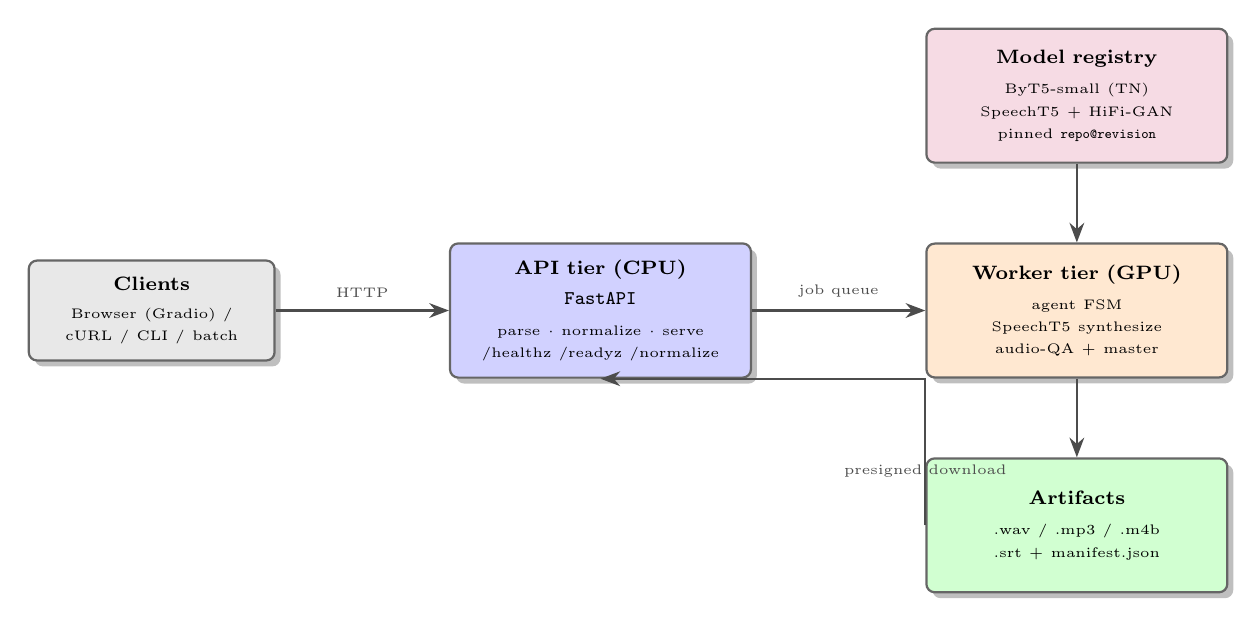
\begin{tikzpicture}[
  node distance=1.0cm and 2.2cm,
  box/.style={rectangle, draw=black!60, rounded corners=3pt, thick,
             text width=3.4cm, minimum height=1.7cm, align=center,
             inner sep=6pt, font=\scriptsize, drop shadow},
  clientbox/.style={box, fill=gray!18, text width=2.7cm, minimum height=1.1cm},
  apibox/.style={box, fill=blue!18},
  workerbox/.style={box, fill=orange!18},
  modelbox/.style={box, fill=purple!14},
  storebox/.style={box, fill=green!18},
  arrow/.style={-{Stealth[length=2.5mm]}, thick, color=black!70}
]

\node[clientbox] (client) {%
  \textbf{Clients}\\[2pt]
  {\tiny Browser (Gradio) / cURL / CLI / batch}
};
\node[apibox, right=of client] (api) {%
  \textbf{API tier (CPU)}\\[3pt]
  \texttt{FastAPI}\\[3pt]
  {\tiny parse $\cdot$ normalize $\cdot$ serve}\\
  {\tiny /healthz /readyz /normalize}
};
\node[workerbox, right=of api] (worker) {%
  \textbf{Worker tier (GPU)}\\[3pt]
  {\tiny agent FSM}\\
  {\tiny SpeechT5 synthesize}\\
  {\tiny audio-QA + master}
};
\node[modelbox, above=1.0cm of worker] (models) {%
  \textbf{Model registry}\\[3pt]
  {\tiny ByT5-small (TN)}\\
  {\tiny SpeechT5 + HiFi-GAN}\\
  {\tiny pinned \texttt{repo@revision}}
};
\node[storebox, below=1.0cm of worker] (store) {%
  \textbf{Artifacts}\\[3pt]
  {\tiny .wav / .mp3 / .m4b}\\
  {\tiny .srt + manifest.json}
};

\draw[arrow] (client.east) -- node[above=1pt, font=\tiny] {HTTP} (api.west);
\draw[arrow] (api.east) -- node[above=1pt, font=\tiny] {job queue} (worker.west);
\draw[arrow] (models.south) -- (worker.north);
\draw[arrow] (worker.south) -- (store.north);
\draw[arrow] (store.west) |- node[below=1pt, font=\tiny, pos=0.25] {presigned download} (api.south);

\end{tikzpicture}%
}
\caption{Two-tier deployment: a CPU API tier (parsing/normalization/serving) is separated from a GPU worker tier (agent FSM + SpeechT5 synthesis + audio-QA + mastering) by a job queue, so synthesis throughput scales by adding GPU workers independently of the frontend. The model registry pins every backend by \texttt{repo@revision}; each job writes a self-contained \texttt{manifest.json}.}
\label{fig:arch}
\end{figure}

\subsection{REST API Endpoints}

\begin{table}[H]
\centering
\caption{FastAPI endpoints (\texttt{src/audiobook\_ai/api/main.py})}
\small
\begin{tabularx}{\linewidth}{@{} l l L @{}}
\toprule
\textbf{Method} & \textbf{Path} & \textbf{Purpose} \\
\midrule
\texttt{GET} & \texttt{/healthz} & Liveness probe (process is up) \\
\texttt{GET} & \texttt{/readyz} & Readiness probe (models loaded) \\
\texttt{POST} & \texttt{/normalize} & Text $\rightarrow$ spoken-form preview (TN model only, no audio) \\
\texttt{POST} & \texttt{/synthesize} & Full synthesis from a JSON body \\
\texttt{POST} & \texttt{/synthesize/file} & Full synthesis from an uploaded document \\
\texttt{GET} & \texttt{/artifacts/...} & Static mount serving generated artifacts \\
\texttt{GET} & \texttt{/download} & Download a produced audiobook / artifact \\
\bottomrule
\end{tabularx}
\end{table}

\paragraph{Example \texttt{POST /normalize}:}
\begin{lstlisting}[basicstyle=\ttfamily\footnotesize]
// request
{ "text": "Dr. Smith paid $5.2M in 1984." }
// response
{
  "input":  "Dr. Smith paid $5.2M in 1984.",
  "spoken": "Doctor Smith paid five point two million dollars in nineteen eighty-four.",
  "confidence": 0.91
}
\end{lstlisting}

\subsection{Latency (RTF) and Scalability}

Latency is reported as the \textbf{Real-Time Factor (RTF)} -- processing time divided by audio duration -- and recorded in \texttt{manifest.json} for every run.

\begin{table}[H]
\centering
\caption{Latency (RTF) -- from the validated end-to-end run}
\begin{tabular}{llL}
\toprule
\textbf{Environment} & \textbf{RTF} & \textbf{Interpretation} \\
\midrule
CPU (validated) & \textbf{2.28} & $\approx$2.28 s of compute per 1 s of audio \\
GPU (estimated) & $\sim$0.1 & $\approx$10$\times$ faster than real time \\
\bottomrule
\end{tabular}
\end{table}

These come from a validated end-to-end run with the real SpeechT5 backend on CPU: 3 chapters, 7 spoken segments, 0 flagged, all 4 agent decisions fired, producing a \textbf{67-second WAV + SRT + manifest} at \textbf{RTF 2.28}. The workload is TTS-bound and parallelizes cleanly at the segment level: \textbf{chunk-level parallelism} (independent segments synthesize concurrently, restored to order at stitch), \textbf{GPU micro-batching} (groups same-voice/same-model segments), and a \textbf{queue-based API/worker split} so synthesis scales by adding GPU workers. \textbf{Time-to-first-audio} is first-class: chapter 1 streams while later chapters render.

\subsection{Model Versioning}

The model registry (\texttt{models/model\_registry.py}) tracks trained TN models via a \texttt{tn\_meta.json} record plus a \texttt{latest} pointer, so the serving layer resolves a known-good normalizer at startup. All pretrained backends are pinned by \textbf{\texttt{repo@revision}} so deployments are reproducible: TN \texttt{google/byt5-small} (Apache-2.0; fallback \texttt{t5-small}), TTS \texttt{microsoft/speecht5\_tts} + \texttt{speecht5\_hifigan} (MIT), speaker x-vectors \texttt{Matthijs/cmu-arctic-xvectors} (MIT). The commercial serving path uses only MIT/Apache ids; non-commercial backends are gated off by default.

\subsection{Packaging: Docker and Hugging Face Space}

Two Docker images -- an \textbf{API image (CPU)} and a \textbf{worker image (GPU)} -- match the tier split; \texttt{docker-compose.yml} wires them with the job queue. The Gradio UI is published as a Hugging Face Space that runs CPU-only (SpeechT5 is CPU-demo-able), with the LLM brain off by default (zero paid API). Where \texttt{ffmpeg} is unavailable the \texttt{.m4b} path degrades gracefully to \texttt{.wav}/\texttt{.mp3}/\texttt{.srt}.

% ============================================================
\section{Agentic AI Component}
\label{sec:agent}
% ============================================================

\subsection{Design Philosophy}

The mandatory agentic component is a \textbf{deterministic finite-state machine (FSM)} over a shared, append-only, versioned \texttt{JobState}. It is \textbf{deterministic-first}: audiobook production must be reproducible, auditable, and runnable CPU-only with zero paid API (the LLM brain is \textbf{off by default}). Every transition is a pure function of the current \texttt{JobState} plus tool outputs, so the same input book yields the same decisions and the same manifest. The optional Anthropic LLM brain is a \emph{bounded escalation path} consulted only at D2; on any failure (no key, timeout, malformed output, low confidence) the FSM \textbf{falls back to the rule normalizer}. The LLM can never take the pipeline off its rails.

\subsection{The Five-Step Pipeline}

States correspond to pipeline stages. Each state runs one or more deterministic \textbf{tools}, writes outputs into \texttt{JobState}, may consult a \textbf{decision point}, and appends a \texttt{ToolTrace} (timing) plus, where applicable, a \texttt{Decision} to the audit log.

\begin{figure}[H]
\centering
\resizebox{\linewidth}{!}{%
\begin{tikzpicture}[
  node distance=0.32cm,
  step/.style={rectangle, draw=black!60, rounded corners=2pt, thick,
              text width=13.5cm, inner sep=5pt, minimum height=0.7cm,
              align=center, font=\footnotesize},
  parse/.style={step, fill=gray!15},
  seg/.style={step, fill=teal!15},
  norm/.style={step, fill=orange!15},
  voice/.style={step, fill=purple!12},
  synth/.style={step, fill=blue!15},
  qa/.style={step, fill=red!12},
  out/.style={step, fill=green!15},
  arrow/.style={-{Stealth[length=2mm]}, thick}
]

\node[parse] (p) {\textbf{1. PARSE + chapter detect} (\textit{tool}): ebooklib / PyMuPDF+pdfplumber / txt+md $\rightarrow$ \texttt{parse\_score} \quad \textbf{[D1]}};
\node[seg, below=of p] (s) {\textbf{2. SEGMENT + CLASSIFY} (\textit{tool}): pysbd sentences + TTS-chunking $\rightarrow$ \texttt{narration | dialogue | heading | skippable}};
\node[norm, below=of s] (n) {\textbf{3. NORMALIZE} (\textit{tool} + \textit{reasoning}): trained ByT5 per segment $\rightarrow$ spoken + confidence \quad \textbf{[D2]} accept / flag / LLM / baseline};
\node[voice, below=of n] (v) {\textbf{4. VOICE-ROUTE} (\textit{decision}): label $\rightarrow$ distinct x-vector index, stable per book \quad \textbf{[D4]}};
\node[synth, below=of v] (y) {\textbf{5a. SYNTHESIZE} (\textit{tool}): SpeechT5 + HiFi-GAN at 16\,kHz with the routed x-vector};
\node[qa, below=of y] (q) {\textbf{5b. AUDIO-QA} (\textit{decision}): empty/NaN, duration ratio, peak, silence \quad \textbf{[D3]} bounded re-synth ($\le$2)};
\node[out, below=of q] (e) {\textbf{6. STITCH + EXPORT} (\textit{tool}): silence gaps, ACX $-18$ LUFS / $-3$ dBTP master $\rightarrow$ wav/mp3/m4b + srt + manifest.json};

\foreach \a/\b in {p/s, s/n, n/v, v/y, y/q, q/e}
  \draw[arrow] (\a) -- (\b);

\end{tikzpicture}%
}
\caption{The deterministic agent FSM. Four decision points (D1--D4) branch on measured quality signals; the assignment requires $\ge$3 and this project has four. Every step is timed (\texttt{ToolTrace}) and every branch recorded (\texttt{Decision}) into \texttt{manifest.json}.}
\label{fig:agent}
\end{figure}

\subsection{Decision Points (D1--D4)}

\begin{table}[H]
\centering
\caption{The four agent decision points (each is a pure function of \texttt{JobState} with an explicit fallback)}
\small
\begin{tabularx}{\linewidth}{@{} l l L @{}}
\toprule
\textbf{ID} & \textbf{Where} & \textbf{Signal, branches, and fallback} \\
\midrule
\textbf{D1} & end of PARSE & \textbf{Parse-quality routing}. \texttt{parse\_score $\in[0,1]$} from alpha-ratio + structure signal + segment-length sanity. $\ge$0.85 $\rightarrow$ \texttt{structured}; 0.5--0.85 $\rightarrow$ \texttt{assisted}; $<$0.5 $\rightarrow$ \texttt{degraded} (flat-text). \emph{Fallback}: the degraded path is itself the graceful floor. \\
\addlinespace
\textbf{D2} & per segment, NORMALIZE & \textbf{Normalization-confidence escalation}. \texttt{confidence} = length-normalized sequence probability; also records neural-vs-baseline disagreement. $\ge$0.55 $\rightarrow$ accept (\texttt{source=neural}); $<$0.55 $\rightarrow$ flag and optionally escalate to the LLM brain (validated). \emph{Fallback}: rule normalizer (\texttt{source=baseline}); LLM off by default. \\
\addlinespace
\textbf{D3} & per clip, AUDIO-QA & \textbf{Audio-QA re-synthesis gate}. Checks: empty/NaN, duration ratio, peak/clipping, silence fraction. On fail $\rightarrow$ bounded re-synth (max 2 attempts), escalating reseed $\rightarrow$ split $\rightarrow$ fallback backend. \emph{Fallback}: accept-best + flag (guarantees forward progress). \\
\addlinespace
\textbf{D4} & VOICE-ROUTE & \textbf{Voice routing}. \texttt{heading / dialogue / narration} $\rightarrow$ distinct CMU-Arctic x-vector indices; the \texttt{voice\_map} is fixed per book for voice stability. \emph{Fallback}: if only one voice is available, all labels collapse to the narrator without failing. \\
\bottomrule
\end{tabularx}
\end{table}

The FSM records \texttt{\{decision, branch, rule\_score, llm\_used, llm\_conf, final\_reason, tool\_version\}} for every firing. The optional LLM brain (\texttt{llm\_advise}, wrapped with \texttt{temperature=0}, an 8\,s timeout, strict-JSON validation, and a payload-hash cache) is consulted only at D2 and always defers to the rule result on any failure.

\subsection{Tool Contracts}

Tools are deterministic functions with explicit pydantic input/output schemas, each emitting a \texttt{ToolTrace}: \texttt{tool\_parse} (text + chapters + labelled segments + \texttt{parse\_score}), \texttt{tool\_normalize} (spoken + confidence + source), \texttt{tool\_route\_voices} (x-vector index), \texttt{tool\_synthesize} (clip + sr; \texttt{strategy} lets D3 reseed/split/swap backend), \texttt{tool\_audio\_qa} (per-clip checks + pass), and \texttt{tool\_stitch} (mastered audio + \texttt{.srt} + \texttt{manifest.json}). The backend fallback chain is SpeechT5 (primary, MIT) $\rightarrow$ optional Kokoro/Parler $\rightarrow$ \texttt{pyttsx3} (offline OS TTS) $\rightarrow$ \texttt{PlaceholderTTS} (deterministic low-noise floor so the pipeline \emph{never} hard-fails and is testable with no model).

\subsection{Worked Example Interaction (the sample book)}

\begin{lstlisting}[basicstyle=\ttfamily\footnotesize]
Input: a short public-domain book; follow one heading, one narration sentence
       with the written date "March 3, 1921", and one line of dialogue.

1) PARSE + D1: ebooklib reads the EPUB, detects a TOC + "Chapter N" headings.
   parse_score = 0.93  ->  D1: 0.93 >= 0.85  ->  parse_mode = structured
   (3 chapters retained). Decision(D1, score=0.93, branch=structured) logged.

2) SEGMENT/CLASSIFY: pysbd splits sentences; chunker labels:
   "Chapter One"                                  -> heading
   "He returned on March 3, 1921, to an empty house." -> narration
   "\"You're late,\" she said."                   -> dialogue

3) NORMALIZE + D2: trained ByT5 runs per segment.
   narration -> "He returned on March third, nineteen twenty-one, to an empty
                 house."   (1921 read as a YEAR; day 3 read as ORDINAL "third"
                            because the model used the date context) conf=0.88
   D2: 0.88 >= 0.55 -> ACCEPT, source=neural. 0 flagged.
   (A context-blind baseline would risk "March three, one thousand nine hundred
    twenty-one" -- exactly the failure the trained model fixes.)

4) VOICE-ROUTE + D4: voice_map = {heading->xv[h], narration->xv[n],
   dialogue->xv[d]} (distinct CMU-Arctic x-vectors), fixed for the whole book.

5) SYNTHESIZE + AUDIO-QA + D3: SpeechT5 + HiFi-GAN renders each clip; the
   narration clip says "nineteen twenty-one". D3: all clips PASS on attempt 1
   -> accept, no re-synth. Decision(D3, pass=true) logged.

6) STITCH + EXPORT: silence gaps, ACX -18 LUFS / -3 dBTP master, chapter markers
   -> .wav / .mp3 / .m4b + .srt. manifest records input_sha256, 3 chapters, each
   segment's source/confidence, all four Decisions, 0 flags, loudness, RTF 2.28.

Net result: every decision fired; the hard NLP case (March 3, 1921 -> "March
third, nineteen twenty-one") was handled by the trained context-aware normalizer;
the agent produced an auditable, mastered audiobook with no human intervention
and no paid API.
\end{lstlisting}

% ============================================================
\section{Continual Learning \& Monitoring}
% ============================================================

\subsection{Monitoring Strategy}

Every pipeline step is timed (\texttt{ToolTrace}) and every decision recorded (\texttt{Decision}) into \texttt{manifest.json}; \texttt{src/audiobook\_ai/monitoring/drift\_report.py} (CLI \texttt{audiobook-ai monitor}) aggregates these signals over a window and diffs them against fixed reference anchors (a frozen golden set, the shipped offline test/hard slices, and the incumbent model during canary/AB).

\begin{table}[H]
\centering
\caption{Monitored signals (each ties to a concrete pipeline mechanism)}
\small
\begin{tabularx}{\linewidth}{@{} l L l @{}}
\toprule
\textbf{Metric} & \textbf{Definition} & \textbf{Concern} \\
\midrule
TN flag-rate & fraction of segments flagged by D2 (conf $<$0.55 or neural-vs-baseline disagreement) & $\uparrow$ bad \\
Audio-QA fail-rate & fraction of clips failing D3 checks and needing re-synth & $\uparrow$ bad \\
RTF drift & Real-Time Factor per run ($\sim$2.28 CPU, $\sim$0.1 GPU) & $\uparrow$ bad \\
Confidence distribution & histogram of length-normalized sequence probabilities & left-shift bad \\
Per-class golden-set accuracy & sentence/class EM per semiotic class on the frozen golden set & $\downarrow$ bad \\
\bottomrule
\end{tabularx}
\end{table}

\subsection{Continual Learning Strategy}

The loop is intentionally circular: production \textbf{flags} (D2/D3) $\rightarrow$ \textbf{feedback store} $\rightarrow$ \textbf{augmented corpus} $\rightarrow$ \textbf{periodic fine-tune} $\rightarrow$ \textbf{registry-versioned canary/AB} $\rightarrow$ \textbf{drift monitoring} $\rightarrow$ new flags.

\begin{enumerate}\setlength\itemsep{0.15em}
  \item \textbf{Collect} new signal automatically per run: low-confidence D2 segments, neural-vs-baseline disagreements, D3 audio-QA failures, and user corrections from the \texttt{/normalize} preview (gold human labels).
  \item \textbf{Assemble} an augmented corpus: regenerated synthetic corpus (extended to cover newly observed token shapes) + human-verified real corrections + the optional DigitalUmuganda sanity set; preserve dedup-before-split and PLAIN $\le$30\%.
  \item \textbf{Fine-tune} with the established recipe (lr 5e-4, effective batch 256, early stopping, \texttt{load\_best\_model\_at\_end}); the held-out hard slice is the canary metric for ambiguity handling.
  \item \textbf{Gate offline}: the candidate must beat the current model on the held-out test and hard slices and must not regress macro per-class accuracy.
  \item \textbf{Canary then A/B}: promote behind the \texttt{latest} pointer for a fraction of books, then run an A/B split to attribute movement to the model rather than input mix.
  \item \textbf{Promote or roll back}: because the registry pins \texttt{repo@revision}, rollback is a one-line pointer change with no image redeploy.
\end{enumerate}

% ============================================================
\section{Data Privacy \& Model Robustness}
% ============================================================

\subsection{Privacy}

PII naturally appears inside books, concentrated in three semiotic classes (\texttt{TELEPHONE}, \texttt{ELECTRONIC}, \texttt{ABBREV}). The guiding principle is \emph{never hard-fail and never leak}:

\begin{itemize}\setlength\itemsep{0.15em}
  \item \textbf{Data minimization}: only what the run needs; intermediate text buffers carrying PII spans are not persisted long-term.
  \item \textbf{No raw PII in logs}: \texttt{ToolTrace}/\texttt{Decision} records carry \emph{metrics and decisions} (parse scores, confidence, disagreement flags, QA verdicts, RTF) -- never the literal phone number or email; segments are referenced by index and class.
  \item \textbf{NER is attribution-scoped}: named entities feed only D4 voice routing and are then discarded -- not written to a ``people in this book'' store.
  \item \textbf{TTL cleanup}: intermediate working data carrying PII is subject to time-to-live cleanup after delivery.
  \item \textbf{Optional redaction / skip}: the \texttt{skippable} label can route sensitive \texttt{TELEPHONE}/\texttt{ELECTRONIC} content to skip or redaction before synthesis.
  \item \textbf{Provenance}: the input file's \textbf{SHA-256} is recorded in the manifest (derivative-work / rights tracking) without retaining the raw content.
\end{itemize}

\subsection{Robustness}

\begin{itemize}\setlength\itemsep{0.15em}
  \item \textbf{Byte-level by design}: ByT5-small operates on raw bytes, so it is robust to numbers, symbols, OOV tokens, typos, and odd formats -- exactly the garbage real documents contain.
  \item \textbf{Trained-for robustness}: the synthetic corpus injects ambiguity and holds out a hard slice; the rule baseline collapses to \texttt{hard = 0.006} EM, which the trained model is built to lift far above.
  \item \textbf{OOD inputs $\rightarrow$ degraded path}: scanned PDFs, garbled OCR, and unsupported languages produce a low \texttt{parse\_score}; D1 routes them to the degraded flat-text path so the system produces \emph{some} audio rather than crashing or emitting nonsense chapters.
  \item \textbf{Defense in depth}: rule guardrail (D2 fallback) + audio-QA re-synth gate (D3) + unrecoverable-error counting guard against hallucinated pronunciations; the TTS backend ladder ends at \texttt{PlaceholderTTS} so the pipeline never hard-fails and is testable with no weights.
\end{itemize}

% ============================================================
\section{Project Management}
% ============================================================

This project was completed \textit{individually}; the workflow simulates team-style planning across seven phases mapped to an eight-week schedule, with phases deliberately overlapping so the synthetic generator and rule baseline stand up early as both training data and an evaluation yardstick.

\begin{table}[H]
\centering
\caption{Project timeline (seven phases over eight weeks)}
\small
\begin{tabularx}{\linewidth}{@{} l l L @{}}
\toprule
\textbf{Week} & \textbf{Phase} & \textbf{Milestone / definition of done} \\
\midrule
W1 & Research \& scoping & Scope locked; VERIFIED ids + licenses (ByT5-small primary, t5-small fallback; SpeechT5 + HiFi-GAN + cmu-arctic-xvectors); commercial path MIT/Apache only \\
W2 & Data \& baseline & \texttt{tn\_corpus.py} emits 60k/4k/4k/1.5k (dedup, leakage-free, PLAIN $\le$30\%); rule baseline built \\
W2--W3 & Data / eval & Baseline EM recorded: easy 0.945 / hard 0.006 / overall 0.712 -- the bar to beat \\
W3--W5 & Model + training & ByT5 trained with \texttt{Seq2SeqTrainer}, anti-overfitting controls; $\approx$3--6 h on one H100 \\
W4--W5 & Agent & FSM with D1--D4, \texttt{ToolTrace}/\texttt{Decision} audit, optional LLM brain (off by default) \\
W5--W6 & Deployment & FastAPI + Gradio UI (\texttt{/ui}) + CLI + Docker (api CPU + worker GPU) + model registry \\
W6--W7 & Evaluation & Beat baseline on both slices; macro/per-class accuracy; unrecoverable count $\rightarrow$0; validated end-to-end run (3 chapters, 7 segments, 0 flagged, all 4 decisions, RTF 2.28 CPU) \\
W7--W8 & Docs, report, slides & README, report, slides, monitoring over \texttt{manifest.json} \\
\bottomrule
\end{tabularx}
\end{table}

\textbf{Scaling reflection.} The module split is the contract between teams. After W2, three workstreams run concurrently because they communicate through stable artifacts, not shared code: \emph{Data + ML} own \texttt{data/$\rightarrow$models/$\rightarrow$training/} (output: a versioned model artifact + metrics); \emph{Backend / Deploy} own \texttt{synthesis/}, \texttt{agent/}, \texttt{api/}, \texttt{deploy/} and consume the model only through the registry; \emph{QA} own \texttt{tests/}, \texttt{analysis/}, \texttt{monitoring/} and define the metric harness up front so ``beats baseline'' and ``unrecoverable rate $\rightarrow$0'' are enforced as gates. The hard interfaces (the \texttt{normalize} step and \texttt{manifest.json}) are already produced by the solo pipeline, so they need no redesign to become team boundaries. A natural fifth workstream (Trust \& Safety / Legal) layers PII handling, voice-cloning consent gating, and per-title rights checks on the same audit trail.

% ============================================================
\section{Ethics \& Responsible AI}
% ============================================================

\subsection{Who Benefits}

Readers with disabilities (spoken access to text-only documents), commuters and time-constrained learners, independent authors (compute-only cost), publishers (faster catalog conversion with chaptered \texttt{.m4b} + \texttt{.srt}), and language learners (synchronized subtitles). The honest framing: the value is \textbf{scale and cost}, not artistic performance -- the system does not claim to match a skilled human narrator.

\subsection{Who Could Be Harmed}

\begin{itemize}\setlength\itemsep{0.15em}
  \item \textbf{Human narrators}: cheap synthetic narration can displace paid voice work -- a labor-displacement risk no technical safeguard fully resolves.
  \item \textbf{Voice-clone misuse}: high-quality cloning backends can reproduce a specific person's voice (impersonation, deepfakes). This is the single most dangerous capability and is treated as such (see safeguards).
  \item \textbf{Copyright holders}: converting a book is a derivative work; at catalog scale the same automation could mass-produce pirated audiobooks.
  \item \textbf{People named inside books}: PII (phones, addresses, emails, names) could be inadvertently persisted by careless logging.
\end{itemize}

\subsection{Bias \& Fairness (named, not hidden)}

\begin{itemize}\setlength\itemsep{0.15em}
  \item \textbf{Narrow voice coverage}: the default voice bank \texttt{Matthijs/cmu-arctic-xvectors} has \textbf{7 speakers} -- a narrow slice of human vocal diversity, so the range of accents/ages/dialects a listener hears is structurally limited.
  \item \textbf{English-/US-centric normalization}: currency-as-dollars, US date ordering, and imperial measure habits bias toward US English; other locales and non-English passages can normalize incorrectly.
  \item \textbf{Name pronunciation}: byte-level ByT5 is robust to OOV \emph{as strings} but does not guarantee culturally correct pronunciation; subtle name mispronunciations may slip below the catastrophic-error threshold.
\end{itemize}

\subsection{Explainability and Misuse Safeguards}

Every reading is \textbf{auditable} without reading code, via three artifacts: the per-segment normalized script (see \texttt{\$5.2M} $\rightarrow$ ``five point two million dollars'' before any audio), the D1--D4 decision log, and the content-hash \texttt{manifest.json}. So a complaint like ``the narrator read my name wrong in chapter 4'' traces to the exact segment, normalization, and voice index. Misuse safeguards: voice-cloning backends (\texttt{coqui/XTTS-v2} CPML, \texttt{SWivid/F5-TTS} CC-BY-NC, \texttt{facebook/mms-tts-eng} CC-BY-NC) are \textbf{non-commercial, consent-gated, and OFF by default}; the input SHA-256 in the manifest is a tamper-evident record of \emph{what} was converted; the commercial path is restricted to MIT/Apache ids by license hygiene, not just policy; and degradation is non-deceptive (a degraded run is flagged, never passed off as clean).

\subsection{Residual Risks Not Claimed Solved}

Labor displacement is an economic harm the deployer must weigh; consent gating is procedural (it cannot verify a claimed consent is genuine); rights verification is the operator's responsibility (the SHA-256 proves \emph{what}, not \emph{that the operator had the right}); voice/locale coverage is narrow; and name pronunciation can still be subtly wrong. Shipping these limits in writing -- alongside an auditable manifest and decision log -- is more ethical than implying the system is neutral, complete, or risk-free.

% ============================================================
\section{Conclusion \& Future Work}
% ============================================================

\subsection{Summary}

\begin{itemize}\setlength\itemsep{0.15em}
  \item Complete end-to-end system: synthetic-corpus build $\rightarrow$ TN training $\rightarrow$ evaluation $\rightarrow$ agentic orchestration $\rightarrow$ deployment $\rightarrow$ monitoring.
  \item The trainable core is a \textbf{ByT5-small} byte-level Text-Normalization model chosen for OOV-free, character-faithful robustness, with a context-blind rule baseline to beat (verified offline: easy 0.945 / \textbf{hard 0.006} / overall 0.712 sentence EM).
  \item A deterministic \textbf{agent FSM} with \textbf{four decision points} (D1--D4): multi-step reasoning (D2 confidence escalation), tool usage (parse/normalize/route/synthesize/QA/stitch), and decision-making on intermediate outputs -- validated end-to-end (3 chapters, 7 segments, 0 flagged, all 4 decisions fired, 67\,s WAV + SRT + manifest, RTF 2.28 CPU).
  \item \textbf{Deployable} four ways (REST API + Gradio UI + CLI + batch) plus Docker and a Hugging Face Space, CPU-only with zero paid API, mastered to ACX $-18$ LUFS / $-3$ dBTP.
  \item License-clean by design: commercial path is MIT/Apache only; non-commercial cloning models are flagged and gated off.
\end{itemize}

\subsection{Future Work}

\begin{enumerate}\setlength\itemsep{0.15em}
  \item \textbf{Scale-up data}: optionally convert the off-Hub Google TN Challenge (16 classes, $\sim$1.1B words) to push per-class accuracy.
  \item \textbf{Quality TTS}: enable Kokoro (24\,kHz, Apache-2.0) and prompt-styled Parler voices behind a toggle for higher naturalness.
  \item \textbf{Word-level alignment}: forced-aligned \texttt{.srt} word timestamps (with a permissive aligner for the commercial path).
  \item \textbf{Consent-gated character voices}: a voice-cast UI with documented consent for any cloned voice (research/demo only).
  \item \textbf{Real-time monitoring}: a drift dashboard over \texttt{manifest.json} with per-class golden-set alerting and canary A/B rollout.
\end{enumerate}

% ============================================================
\newpage
\begin{thebibliography}{9}

\bibitem{abogen} \c{S}afak, D. \textit{abogen} -- audiobook generation (reference inspiration). GitHub. \url{https://github.com/denizsafak/abogen}

\bibitem{byt5} Xue, L., et al. (2022). ByT5: Towards a Token-Free Future with Pre-trained Byte-to-Byte Models. \textit{TACL}.

\bibitem{t5} Raffel, C., et al. (2020). Exploring the Limits of Transfer Learning with a Unified Text-to-Text Transformer (T5). \textit{JMLR 21}.

\bibitem{sproat} Sproat, R., \& Jaitly, N. (2016). RNN Approaches to Text Normalization: A Challenge. \textit{arXiv:1611.00068}.

\bibitem{speecht5} Ao, J., et al. (2022). SpeechT5: Unified-Modal Encoder-Decoder Pre-training for Spoken Language Processing. \textit{ACL 2022}.

\bibitem{huggingface} Wolf, T., et al. (2020). Transformers: State-of-the-Art Natural Language Processing. \textit{EMNLP 2020}.

\bibitem{fastapi} Ram\'irez, S. (2018). FastAPI. \url{https://fastapi.tiangolo.com/}

\bibitem{pysbd} Sadvilkar, N., \& Neumann, M. (2020). PySBD: Pragmatic Sentence Boundary Disambiguation. \textit{EMNLP 2020 (NLP-OSS)}.

\bibitem{num2words} Ogawa, T., et al. \textit{num2words}: number-to-words verbalization library. \url{https://github.com/savoirfairelinux/num2words}

\bibitem{acx} Audiobook Creation Exchange (ACX). \textit{Audio Submission Requirements} ($-18$ to $-23$ LUFS, $-3$ dBTP peak).

\end{thebibliography}

\end{document}
